% Bab 2: Regular Expression dan Finite Automata untuk Lexical Analysis
% File ini dapat dikompilasi terpisah atau sebagai bagian dari main.tex

\chapter[Regular Expression dan Finite Automata]{Regular Expression dan Finite Automata\\untuk Lexical Analysis}
\label{chap:regex-fa}

\section{Tujuan Pembelajaran}

Setelah mempelajari bab ini, mahasiswa diharapkan mampu:
\begin{enumerate}
    \item Memahami konsep regular expression dan regular language
    \item Menjelaskan perbedaan antara NFA (Nondeterministic Finite Automata) dan DFA (Deterministic Finite Automata)
    \item Mengkonversi regular expression ke NFA menggunakan algoritma Thompson
    \item Mengkonversi NFA ke DFA menggunakan subset construction
    \item Mengimplementasikan NFA dan DFA sederhana dalam C/C++
    \item Membuat recognizer untuk pattern token sederhana menggunakan finite automata
    \item Memahami hubungan antara regular expression, finite automata, dan lexical analysis
\end{enumerate}

\section{Pendahuluan}

Sebagai landasan untuk memahami lexical analysis, kita perlu mempelajari teori formal yang mendasarinya. Menurut sumber dari Aoyama Gakuin University:

\begin{quote}
``Lexical analysis breaks input text into lexemes which correspond to tokens. Usually implemented using regular languages → regex → NFA → DFA → (minimized) DFA for efficiency.''\cite{aoyama2024lexical}
\end{quote}

Alur ini menunjukkan bahwa lexical analysis dalam kompilator modern menggunakan teori formal language, khususnya regular languages, yang direpresentasikan sebagai regular expressions dan kemudian diimplementasikan sebagai finite automata untuk efisiensi.

Gambar \ref{fig:lexical-theory-overview} menunjukkan alur lengkap dari regular expression hingga implementasi praktis dalam lexical analyzer.

\begin{figure}[H]
    \centering
    \adjustbox{max width=0.9\textwidth,center}{%
    \begin{tikzpicture}[
        box/.style={rectangle, draw=blue!50, fill=blue!10, text width=1.8cm, text centered, minimum height=0.8cm, rounded corners, font=\footnotesize, inner sep=4pt, align=center},
        arrow/.style={->, >=stealth, thick},
        label/.style={font=\tiny, above, align=center},
        node distance=1.8cm
    ]
    
    \node[box] (regex) {Regular\\Expression};
    \node[box, right=of regex] (nfa) {$\epsilon$-NFA\\(Thompson)};
    \node[box, right=of nfa] (dfa) {DFA\\(Subset)};
    \node[box, right=of dfa] (min) {Minimized\\DFA};
    \node[box, right=of min] (impl) {Scanner};
    
    \draw[arrow] (regex) -- node[label, align=center] {Algoritma\\Thompson} (nfa);
    \draw[arrow] (nfa) -- node[label, align=center] {Subset\\Construction} (dfa);
    \draw[arrow] (dfa) -- node[label] {Minimization} (min);
    \draw[arrow] (min) -- node[label, align=center] {Code\\Generation} (impl);
    
    \end{tikzpicture}%
    }
    \caption{Alur konversi dari regular expression ke implementasi scanner}
    \label{fig:lexical-theory-overview}
\end{figure}

\section{Regular Expression dan Regular Language}

\subsection{Definisi Regular Expression}

Regular expression (regex) adalah notasi formal untuk mendeskripsikan pola string dalam suatu bahasa. Regular expression menggunakan operasi-operasi dasar untuk membangun pattern yang lebih kompleks.

Operasi-operasi dasar dalam regular expression meliputi:

\begin{enumerate}
    \item \textbf{Literal}: Karakter tunggal, misalnya \texttt{a} mencocokkan string ``a''
    \item \textbf{Concatenation}: Penggabungan, misalnya \texttt{ab} mencocokkan string ``ab''
    \item \textbf{Union/Alternation}: Pilihan, misalnya \texttt{a|b} mencocokkan ``a'' atau ``b''
    \item \textbf{Kleene Star}: Nol atau lebih pengulangan, misalnya \texttt{a*} mencocokkan ``'', ``a'', ``aa'', ``aaa'', dll.
    \item \textbf{Kleene Plus}: Satu atau lebih pengulangan, misalnya \texttt{a+} mencocokkan ``a'', ``aa'', ``aaa'', dll.
    \item \textbf{Optional}: Nol atau satu, misalnya \texttt{a?} mencocokkan ``'' atau ``a''
    \item \textbf{Character Class}: Set karakter, misalnya \texttt{[0-9]} mencocokkan digit 0-9
\end{enumerate}

\subsection{Contoh Regular Expression untuk Token}

Dalam lexical analysis, setiap jenis token didefinisikan menggunakan regular expression. Berikut beberapa contoh:

\begin{itemize}
    \item \textbf{Identifier}: \texttt{[a-zA-Z\_][a-zA-Z0-9\_]*}
    \begin{itemize}
        \item Dimulai dengan huruf atau underscore
        \item Diikuti oleh nol atau lebih huruf, digit, atau underscore
    \end{itemize}
    
    \item \textbf{Integer Literal}: \texttt{[0-9]+}
    \begin{itemize}
        \item Satu atau lebih digit
    \end{itemize}
    
    \item \textbf{Floating Point}: \texttt{[0-9]+\textbackslash.[0-9]+}
    \begin{itemize}
        \item Digit, titik desimal, digit
    \end{itemize}
    
    \item \textbf{String Literal}: \texttt{"([\textasciicircum"\\]|\textbackslash\textbackslash.)*"}
    \begin{itemize}
        \item Dimulai dan diakhiri dengan tanda kutip
        \item Berisi karakter apapun kecuali tanda kutip (atau escape sequence)
    \end{itemize}
    
    \item \textbf{Whitespace}: \texttt{[ \textbackslash t\textbackslash n]+}
    \begin{itemize}
        \item Satu atau lebih spasi, tab, atau newline
    \end{itemize}
    
    \item \textbf{Operator}: \texttt{+|-|*|/|=|==|!=}
    \begin{itemize}
        \item Operator aritmatika dan perbandingan
    \end{itemize}
\end{itemize}

\subsection{Regular Language}

Bahasa yang dapat dinyatakan dengan regular expression disebut \textbf{regular language}. Regular language memiliki sifat-sifat penting:

\begin{itemize}
    \item Dapat dikenali oleh finite automata (NFA atau DFA)
    \item Tertutup terhadap operasi union, concatenation, dan Kleene star
    \item Tidak dapat mengekspresikan struktur nested (seperti matching parentheses)
    \item Cukup untuk mendeskripsikan sebagian besar token dalam bahasa pemrograman
\end{itemize}

\section{Finite Automata}

Finite automata adalah model matematika yang digunakan untuk mengenali string dalam suatu bahasa. Terdapat dua jenis utama: NFA (Nondeterministic Finite Automata) dan DFA (Deterministic Finite Automata).

\subsection{Definisi Formal}

\textbf{Finite Automaton} didefinisikan sebagai tuple $(Q, \Sigma, \delta, q_0, F)$ dimana:
\begin{itemize}
    \item $Q$: Himpunan state (keadaan) yang terbatas
    \item $\Sigma$: Alphabet (himpunan simbol input)
    \item $\delta$: Fungsi transisi (transition function)
    \item $q_0$: Start state (state awal)
    \item $F$: Himpunan accept states (final states)
\end{itemize}

\subsection{NFA (Nondeterministic Finite Automata)}

NFA memiliki karakteristik:
\begin{itemize}
    \item Untuk suatu state dan input symbol, dapat memiliki \textbf{nol, satu, atau lebih} transisi
    \item Dapat memiliki \textbf{$\epsilon$-transitions} (epsilon transitions) yang tidak mengonsumsi input
    \item Lebih mudah dikonstruksi dari regular expression
    \item Simulasi memerlukan backtracking atau multiple states tracking
\end{itemize}

Contoh NFA untuk pattern \texttt{a|b}:

Gambar \ref{fig:nfa-union} menunjukkan NFA untuk pattern \texttt{a|b} yang menggunakan $\epsilon$-transitions untuk branching.

\begin{figure}[H]
    \centering
    \adjustbox{max width=0.7\textwidth,center}{%
    \begin{tikzpicture}[
        state/.style={circle, draw=blue!50, fill=blue!10, minimum size=0.8cm, font=\footnotesize},
        accept/.style={circle, draw=green!50, fill=green!10, minimum size=0.8cm, font=\footnotesize, double},
        start/.style={circle, draw=red!50, fill=red!10, minimum size=0.8cm, font=\footnotesize},
        arrow/.style={->, >=stealth, thick},
        eps/.style={->, >=stealth, thick, dashed, blue!70},
        node distance=1.5cm and 2cm
    ]
    
    % Start state
    \node[start] (q0) at (0,0) {$q_0$};
    
    % Accept states
    \node[accept] (q1) at (-2,-2) {$q_1$};
    \node[accept] (q2) at (2,-2) {$q_2$};
    
    % Epsilon transitions
    \draw[eps] (q0) to[out=225, in=90] node[left, font=\tiny] {$\epsilon$} (q1);
    \draw[eps] (q0) to[out=315, in=90] node[right, font=\tiny] {$\epsilon$} (q2);
    
    % Symbol transitions
    \draw[arrow] (q1) to[loop left] node[left, font=\tiny] {$a$} (q1);
    \draw[arrow] (q2) to[loop right] node[right, font=\tiny] {$b$} (q2);
    
    % Labels
    \node[above=0.2cm of q0, font=\small] {\textbf{Start}};
    \node[below=0.2cm of q1, font=\tiny] {\textbf{Accept}};
    \node[below=0.2cm of q2, font=\tiny] {\textbf{Accept}};
    
    \end{tikzpicture}%
    }
    \caption{NFA untuk pattern \texttt{a|b} dengan $\epsilon$-transitions}
    \label{fig:nfa-union}
\end{figure}

State $q_0$ adalah start state, $q_1$ dan $q_2$ adalah accept states. Dari $q_0$, dengan $\epsilon$-transition dapat menuju $q_1$ atau $q_2$, kemudian dari $q_1$ dapat menerima 'a', dan dari $q_2$ dapat menerima 'b'.

\subsection{DFA (Deterministic Finite Automata)}

DFA memiliki karakteristik:
\begin{itemize}
    \item Untuk setiap state dan input symbol, terdapat \textbf{tepat satu} transisi
    \item Tidak memiliki $\epsilon$-transitions
    \item Lebih efisien untuk simulasi (deterministic)
    \item Setiap NFA dapat dikonversi menjadi DFA yang ekuivalen
\end{itemize}

Contoh DFA untuk pattern \texttt{a|b}:

Gambar \ref{fig:dfa-union} menunjukkan DFA yang ekuivalen dengan NFA di atas, tetapi deterministik.

\begin{figure}[H]
    \centering
    \adjustbox{max width=0.6\textwidth,center}{%
    \begin{tikzpicture}[
        state/.style={circle, draw=blue!50, fill=blue!10, minimum size=0.8cm, font=\footnotesize},
        accept/.style={circle, draw=green!50, fill=green!10, minimum size=0.8cm, font=\footnotesize, double},
        start/.style={circle, draw=red!50, fill=red!10, minimum size=0.8cm, font=\footnotesize},
        arrow/.style={->, >=stealth, thick},
        node distance=2cm
    ]
    
    % Start state
    \node[start] (q0) at (0,0) {$q_0$};
    
    % Accept states
    \node[accept] (q1) at (-2,-2) {$q_1$};
    \node[accept] (q2) at (2,-2) {$q_2$};
    
    % Transitions
    \draw[arrow] (q0) to[out=225, in=90] node[left, font=\tiny] {$a$} (q1);
    \draw[arrow] (q0) to[out=315, in=90] node[right, font=\tiny] {$b$} (q2);
    
    % Self loops
    \draw[arrow] (q1) to[loop left] node[left, font=\tiny] {$a$} (q1);
    \draw[arrow] (q2) to[loop right] node[right, font=\tiny] {$b$} (q2);
    
    % Labels
    \node[above=0.2cm of q0, font=\small] {\textbf{Start}};
    \node[below=0.2cm of q1, font=\tiny] {\textbf{Accept}};
    \node[below=0.2cm of q2, font=\tiny] {\textbf{Accept}};
    
    \end{tikzpicture}%
    }
    \caption{DFA untuk pattern \texttt{a|b} (deterministik)}
    \label{fig:dfa-union}
\end{figure}

DFA ini deterministik: dari $q_0$, input 'a' selalu menuju $q_1$, input 'b' selalu menuju $q_2$. Tidak ada $\epsilon$-transitions dan setiap state memiliki tepat satu transisi untuk setiap input symbol.

\subsection{Perbedaan NFA dan DFA}

Perbedaan utama antara NFA dan DFA dapat dilihat pada Tabel \ref{tab:nfa-dfa} dan perbandingan visual pada Gambar \ref{fig:nfa-dfa-comparison}.

\begin{table}[H]
\centering
\begin{tabularx}{\textwidth}{|l|X|X|}
\hline
\textbf{Aspek} & \textbf{NFA} & \textbf{DFA} \\
\hline
Transisi per state & Bisa 0, 1, atau lebih & Tepat 1 \\
\hline
$\epsilon$-transitions & Diizinkan & Tidak diizinkan \\
\hline
Efisiensi simulasi & Perlu backtracking & Linear time \\
\hline
Jumlah states & Biasanya lebih sedikit & Bisa lebih banyak \\
\hline
Konstruksi dari regex & Lebih mudah & Lebih kompleks \\
\hline
\end{tabularx}
\caption{Perbandingan NFA dan DFA}
\label{tab:nfa-dfa}
\end{table}

\begin{figure}[H]
    \centering
    \adjustbox{max width=0.9\textwidth,center}{%
    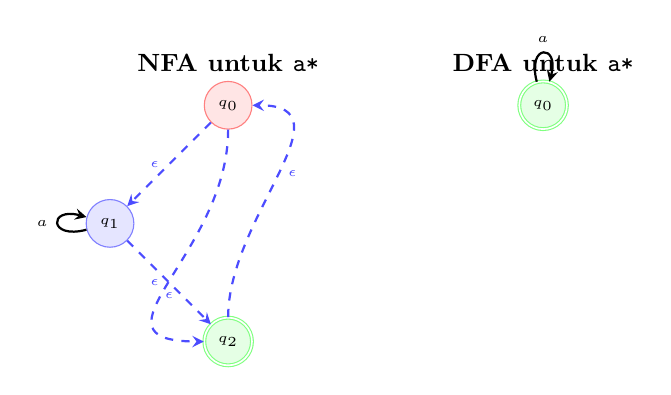
\begin{tikzpicture}[
        state/.style={circle, draw=blue!50, fill=blue!10, minimum size=0.6cm, font=\tiny},
        accept/.style={circle, draw=green!50, fill=green!10, minimum size=0.6cm, font=\tiny, double},
        start/.style={circle, draw=red!50, fill=red!10, minimum size=0.6cm, font=\tiny},
        arrow/.style={->, >=stealth, thick},
        eps/.style={->, >=stealth, thick, dashed, blue!70},
        node distance=1.2cm
    ]
    
    % NFA side
    \node[font=\small\bfseries, above=0.3cm] at (-2,0) {NFA untuk \texttt{a*}};
    \node[start] (nq0) at (-2,0) {$q_0$};
    \node[state] (nq1) at (-3.5,-1.5) {$q_1$};
    \node[accept] (nq2) at (-2,-3) {$q_2$};
    
    \draw[eps] (nq0) -- node[left, font=\tiny] {$\epsilon$} (nq1);
    \draw[arrow] (nq1) to[loop left] node[left, font=\tiny] {$a$} (nq1);
    \draw[eps] (nq1) -- node[left, font=\tiny] {$\epsilon$} (nq2);
    \draw[eps] (nq0) to[out=270, in=180, looseness=1.5] node[below, font=\tiny] {$\epsilon$} (nq2);
    \draw[eps] (nq2) to[out=90, in=0, looseness=1.2] node[right, font=\tiny] {$\epsilon$} (nq0);
    
    % DFA side
    \node[font=\small\bfseries, above=0.3cm] at (2,0) {DFA untuk \texttt{a*}};
    \node[start,accept] (dq0) at (2,0) {$q_0$};
    
    \draw[arrow] (dq0) to[loop above] node[above, font=\tiny] {$a$} (dq0);
    
    \end{tikzpicture}%
    }
    \caption{Perbandingan visual NFA dan DFA untuk pattern \texttt{a*} (keduanya ekuivalen)}
    \label{fig:nfa-dfa-comparison}
\end{figure}

\section{Konversi Regular Expression ke NFA: Algoritma Thompson}

Algoritma Thompson adalah metode sistematis untuk mengkonversi regular expression menjadi $\epsilon$-NFA. Algoritma ini menggunakan pendekatan rekursif dengan template untuk setiap operasi regex.

\subsection{Template Dasar}

Algoritma Thompson menggunakan template untuk setiap operasi regex. Template-template berikut menunjukkan konstruksi dasar yang digunakan.

\subsubsection{Literal (Karakter Tunggal)}

Untuk regex \texttt{a}, NFA-nya adalah:

\begin{figure}[H]
    \centering
    \adjustbox{max width=0.5\textwidth,center}{%
    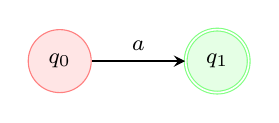
\begin{tikzpicture}[
        state/.style={circle, draw=blue!50, fill=blue!10, minimum size=0.8cm, font=\footnotesize},
        accept/.style={circle, draw=green!50, fill=green!10, minimum size=0.8cm, font=\footnotesize, double},
        start/.style={circle, draw=red!50, fill=red!10, minimum size=0.8cm, font=\footnotesize},
        arrow/.style={->, >=stealth, thick},
        node distance=2cm
    ]
    
    \node[start] (q0) at (0,0) {$q_0$};
    \node[accept] (q1) at (2,0) {$q_1$};
    \draw[arrow] (q0) -- node[above, font=\footnotesize] {$a$} (q1);
    
    \end{tikzpicture}%
    }
    \caption{Template NFA untuk literal \texttt{a}}
    \label{fig:thompson-literal}
\end{figure}

\subsubsection{Concatenation (RS)}

Untuk regex \texttt{RS}, NFA-nya dibangun dengan menghubungkan NFA untuk R dan S menggunakan $\epsilon$-transition:

\begin{figure}[H]
    \centering
    \adjustbox{max width=0.8\textwidth,center}{%
    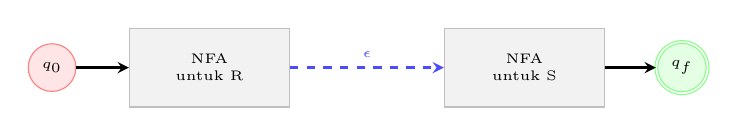
\begin{tikzpicture}[
        state/.style={circle, draw=blue!50, fill=blue!10, minimum size=0.6cm, font=\tiny},
        accept/.style={circle, draw=green!50, fill=green!10, minimum size=0.6cm, font=\tiny, double},
        start/.style={circle, draw=red!50, fill=red!10, minimum size=0.6cm, font=\tiny},
        box/.style={rectangle, draw=gray!50, fill=gray!10, text width=1.8cm, minimum height=1cm, font=\tiny, align=center},
        arrow/.style={->, >=stealth, thick},
        eps/.style={->, >=stealth, thick, dashed, blue!70},
        node distance=1.5cm
    ]
    
    \node[start] (q0) at (0,0) {$q_0$};
    \node[box] (nfaR) at (2,0) {NFA\\untuk R};
    \node (q1) at (4,0) {};
    \node[box] (nfaS) at (6,0) {NFA\\untuk S};
    \node[accept] (qf) at (8,0) {$q_f$};
    
    \draw[arrow] (q0) -- (nfaR);
    \draw[eps] (nfaR) -- node[above, font=\tiny] {$\epsilon$} (nfaS);
    \draw[arrow] (nfaS) -- (qf);
    
    \end{tikzpicture}%
    }
    \caption{Template NFA untuk concatenation \texttt{RS}}
    \label{fig:thompson-concat}
\end{figure}

\subsubsection{Union (R|S)}

Untuk regex \texttt{R|S}, NFA-nya menggunakan $\epsilon$-transitions untuk branching:

\begin{figure}[H]
    \centering
    \adjustbox{max width=0.7\textwidth,center}{%
    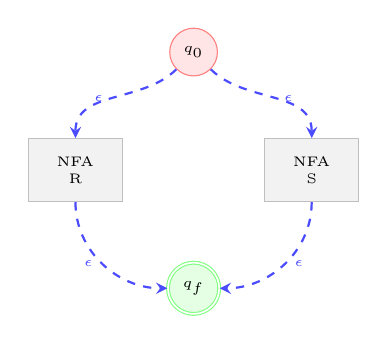
\begin{tikzpicture}[
        state/.style={circle, draw=blue!50, fill=blue!10, minimum size=0.6cm, font=\tiny},
        accept/.style={circle, draw=green!50, fill=green!10, minimum size=0.6cm, font=\tiny, double},
        start/.style={circle, draw=red!50, fill=red!10, minimum size=0.6cm, font=\tiny},
        box/.style={rectangle, draw=gray!50, fill=gray!10, minimum width=1.2cm, minimum height=0.8cm, font=\tiny, align=center},
        arrow/.style={->, >=stealth, thick},
        eps/.style={->, >=stealth, thick, dashed, blue!70},
        node distance=1.2cm
    ]
    
    \node[start] (q0) at (0,0) {$q_0$};
    \node[box] (nfaR) at (-1.5,-1.5) {NFA\\R};
    \node[box] (nfaS) at (1.5,-1.5) {NFA\\S};
    \node[accept] (qf) at (0,-3) {$q_f$};
    
    \draw[eps] (q0) to[out=225, in=90] node[left, font=\tiny] {$\epsilon$} (nfaR);
    \draw[eps] (q0) to[out=315, in=90] node[right, font=\tiny] {$\epsilon$} (nfaS);
    \draw[eps] (nfaR) to[out=270, in=180] node[left, font=\tiny] {$\epsilon$} (qf);
    \draw[eps] (nfaS) to[out=270, in=0] node[right, font=\tiny] {$\epsilon$} (qf);
    
    \end{tikzpicture}%
    }
    \caption{Template NFA untuk union \texttt{R|S}}
    \label{fig:thompson-union}
\end{figure}

\subsubsection{Kleene Star (R*)}

Untuk regex \texttt{R*}, NFA-nya memiliki loop dengan $\epsilon$-transitions:

\begin{figure}[H]
    \centering
    \adjustbox{max width=0.6\textwidth,center}{%
    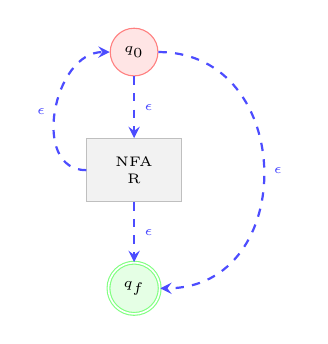
\begin{tikzpicture}[
        state/.style={circle, draw=blue!50, fill=blue!10, minimum size=0.6cm, font=\tiny},
        accept/.style={circle, draw=green!50, fill=green!10, minimum size=0.6cm, font=\tiny, double},
        start/.style={circle, draw=red!50, fill=red!10, minimum size=0.6cm, font=\tiny},
        box/.style={rectangle, draw=gray!50, fill=gray!10, minimum width=1.2cm, minimum height=0.8cm, font=\tiny, align=center},
        arrow/.style={->, >=stealth, thick},
        eps/.style={->, >=stealth, thick, dashed, blue!70},
        node distance=1.5cm
    ]
    
    \node[start] (q0) at (0,0) {$q_0$};
    \node[box] (nfaR) at (0,-1.5) {NFA\\R};
    \node[accept] (qf) at (0,-3) {$q_f$};
    
    % Epsilon transitions
    \draw[eps] (q0) -- node[right, font=\tiny] {$\epsilon$} (nfaR);
    \draw[eps] (nfaR) -- node[right, font=\tiny] {$\epsilon$} (qf);
    
    % Loop transitions
    \draw[eps] (q0) to[out=0, in=0, looseness=1.5] node[right, font=\tiny] {$\epsilon$} (qf);
    \draw[eps] (nfaR) to[out=180, in=180, looseness=1.2] node[left, font=\tiny] {$\epsilon$} (q0);
    
    \end{tikzpicture}%
    }
    \caption{Template NFA untuk Kleene star \texttt{R*}}
    \label{fig:thompson-kleene}
\end{figure}

\subsection{Contoh: Konversi \texttt{(a|b)*abb}}

Mari kita konstruksi NFA untuk regex \texttt{(a|b)*abb} menggunakan algoritma Thompson. Gambar \ref{fig:thompson-example} menunjukkan proses konstruksi langkah demi langkah.

\begin{enumerate}
    \item \textbf{Literal 'a' dan 'b'}: Buat NFA untuk masing-masing
    \item \textbf{Union (a|b)}: Gabungkan dengan $\epsilon$-transitions
    \item \textbf{Kleene Star ((a|b)*)}: Tambahkan loop dengan $\epsilon$-transitions
    \item \textbf{Concatenation dengan 'a'}: Tambahkan NFA untuk 'a'
    \item \textbf{Concatenation dengan 'b'}: Tambahkan NFA untuk 'b' (dua kali)
\end{enumerate}

\begin{figure}[H]
    \centering
    \adjustbox{max width=0.9\textwidth,center}{%
    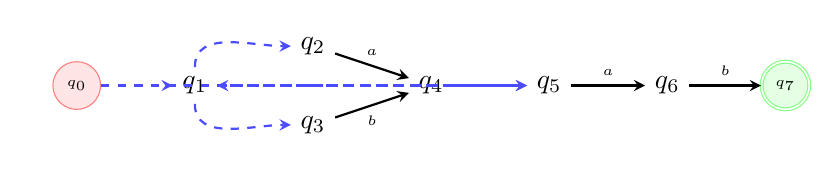
\begin{tikzpicture}[
        state/.style={circle, draw=blue!50, fill=blue!10, minimum size=0.5cm, font=\tiny},
        accept/.style={circle, draw=green!50, fill=green!10, minimum size=0.5cm, font=\tiny, double},
        start/.style={circle, draw=red!50, fill=red!10, minimum size=0.5cm, font=\tiny},
        arrow/.style={->, >=stealth, thick},
        eps/.style={->, >=stealth, thick, dashed, blue!70},
        node distance=0.8cm
    ]
    
    % Start
    \node[start] (q0) at (0,0) {$q_0$};
    
    % (a|b)* part
    \node (q1) at (1.5,0) {$q_1$};
    \node (q2) at (3,0.5) {$q_2$};
    \node (q3) at (3,-0.5) {$q_3$};
    \node (q4) at (4.5,0) {$q_4$};
    
    % 'a' part
    \node (q5) at (6,0) {$q_5$};
    
    % 'b' parts
    \node (q6) at (7.5,0) {$q_6$};
    \node[accept] (q7) at (9,0) {$q_7$};
    
    % Transitions for (a|b)*
    \draw[eps] (q0) -- (q1);
    \draw[eps] (q1) to[out=90, in=180] (q2);
    \draw[eps] (q1) to[out=270, in=180] (q3);
    \draw[arrow] (q2) -- node[above, font=\tiny] {$a$} (q4);
    \draw[arrow] (q3) -- node[below, font=\tiny] {$b$} (q4);
    \draw[eps] (q4) to[out=0, in=0, looseness=2] (q1);
    \draw[eps] (q4) -- (q5);
    
    % 'a' transition
    \draw[arrow] (q5) -- node[above, font=\tiny] {$a$} (q6);
    
    % 'b' transitions
    \draw[arrow] (q6) -- node[above, font=\tiny] {$b$} (q7);
    
    % Direct path from start to accept (for empty string)
    \draw[eps] (q0) to[out=0, in=180, looseness=3] (q5);
    
    \end{tikzpicture}%
    }
    \caption{NFA untuk regex \texttt{(a|b)*abb} menggunakan algoritma Thompson}
    \label{fig:thompson-example}
\end{figure}

Hasil akhirnya adalah NFA yang dapat mengenali string seperti ``abb'', ``aabb'', ``babb'', ``ababb'', dll. NFA ini memiliki $\epsilon$-transitions yang memungkinkan multiple paths untuk input yang sama.

\section{Konversi NFA ke DFA: Subset Construction}

Karena NFA tidak deterministik dan simulasi NFA bisa tidak efisien, kita perlu mengkonversi NFA menjadi DFA yang ekuivalen menggunakan algoritma \textbf{subset construction}.

\subsection{Konsep \texorpdfstring{$\epsilon$}{epsilon}-Closure}

Sebelum subset construction, kita perlu memahami konsep \textbf{$\epsilon$-closure}:

\begin{itemize}
    \item \textbf{$\epsilon$-closure} dari suatu state adalah himpunan semua state yang dapat dicapai dari state tersebut melalui $\epsilon$-transitions saja
    \item \textbf{$\epsilon$-closure} dari suatu set states adalah union dari $\epsilon$-closure setiap state dalam set tersebut
\end{itemize}

\subsection{Algoritma Subset Construction}

Algoritma subset construction bekerja sebagai berikut:

\begin{enumerate}
    \item \textbf{Start State DFA}: $\epsilon$-closure dari start state NFA
    \item \textbf{Untuk setiap state DFA dan setiap input symbol}:
    \begin{enumerate}
        \item Hitung semua NFA states yang dapat dicapai dengan input symbol tersebut
        \item Ambil $\epsilon$-closure dari set states tersebut
        \item Jika hasilnya belum ada sebagai state DFA, buat state baru
        \item Tambahkan transisi dari state DFA saat ini ke state hasil
    \end{enumerate}
    \item \textbf{Accept States DFA}: Setiap state DFA yang mengandung accept state NFA
\end{enumerate}

\subsection{Contoh: Konversi NFA \texttt{(a|b)*abb} ke DFA}

Mari kita ikuti langkah-langkah subset construction. Gambar \ref{fig:subset-construction} menunjukkan proses konversi dan hasil DFA yang dihasilkan.

\begin{enumerate}
    \item \textbf{Start State DFA}: 
    \begin{itemize}
        \item Mulai dari start state NFA, ambil $\epsilon$-closure
        \item Misalkan hasilnya adalah set $\{q_0, q_1, q_4\}$ → ini menjadi state DFA $A$
    \end{itemize}
    
    \item \textbf{Transisi dari State A dengan input 'a'}:
    \begin{itemize}
        \item Dari semua NFA states dalam A, cari yang dapat menerima 'a'
        \item Ambil $\epsilon$-closure dari hasilnya → misalkan $\{q_2, q_4, q_5\}$ → state DFA $B$
    \end{itemize}
    
    \item \textbf{Transisi dari State A dengan input 'b'}:
    \begin{itemize}
        \item Dari semua NFA states dalam A, cari yang dapat menerima 'b'
        \item Ambil $\epsilon$-closure dari hasilnya → misalkan $\{q_3, q_4\}$ → state DFA $C$
    \end{itemize}
    
    \item \textbf{Lanjutkan untuk state B dan C} dengan cara yang sama
    \item \textbf{Accept States}: State DFA yang mengandung accept state NFA (misalnya state yang mengandung $q_7$)
\end{enumerate}

\begin{figure}[H]
    \centering
    \adjustbox{max width=0.85\textwidth,center}{%
    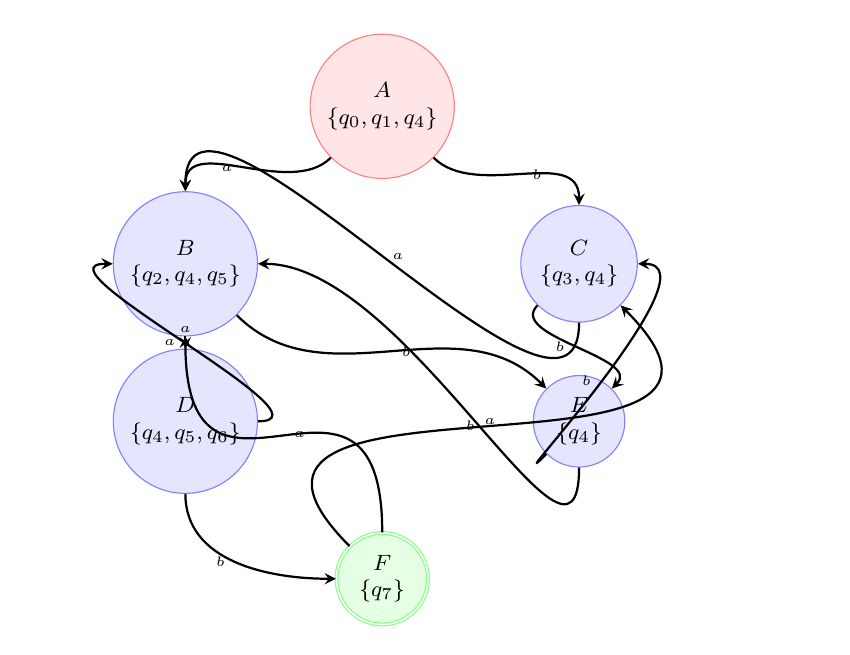
\begin{tikzpicture}[
        state/.style={circle, draw=blue!50, fill=blue!10, minimum size=0.7cm, font=\footnotesize, align=center},
        accept/.style={circle, draw=green!50, fill=green!10, minimum size=0.7cm, font=\footnotesize, double, align=center},
        start/.style={circle, draw=red!50, fill=red!10, minimum size=0.7cm, font=\footnotesize, align=center},
        arrow/.style={->, >=stealth, thick},
        node distance=2.5cm and 2cm
    ]
    
    % DFA States
    \node[start] (A) at (0,0) {$A$\\$\{q_0,q_1,q_4\}$};
    \node[state] (B) at (-2.5,-2) {$B$\\$\{q_2,q_4,q_5\}$};
    \node[state] (C) at (2.5,-2) {$C$\\$\{q_3,q_4\}$};
    \node[state] (D) at (-2.5,-4) {$D$\\$\{q_4,q_5,q_6\}$};
    \node[state] (E) at (2.5,-4) {$E$\\$\{q_4\}$};
    \node[accept] (F) at (0,-6) {$F$\\$\{q_7\}$};
    
    % Transitions
    \draw[arrow] (A) to[out=225, in=90] node[left, font=\tiny] {$a$} (B);
    \draw[arrow] (A) to[out=315, in=90] node[right, font=\tiny] {$b$} (C);
    \draw[arrow] (B) to[out=270, in=90] node[left, font=\tiny] {$a$} (D);
    \draw[arrow] (B) to[out=315, in=135] node[right, font=\tiny] {$b$} (E);
    \draw[arrow] (C) to[out=270, in=90] node[right, font=\tiny] {$a$} (B);
    \draw[arrow] (C) to[out=225, in=45] node[left, font=\tiny] {$b$} (E);
    \draw[arrow] (D) to[out=270, in=180] node[left, font=\tiny] {$b$} (F);
    \draw[arrow] (D) to[out=0, in=180] node[above, font=\tiny] {$a$} (B);
    \draw[arrow] (E) to[out=270, in=0] node[right, font=\tiny] {$a$} (B);
    \draw[arrow] (E) to[out=225, in=0] node[left, font=\tiny] {$b$} (C);
    \draw[arrow] (F) to[out=90, in=270, looseness=2] node[right, font=\tiny] {$a$} (B);
    \draw[arrow] (F) to[out=135, in=315, looseness=2] node[left, font=\tiny] {$b$} (C);
    
    \end{tikzpicture}%
    }
    \caption{DFA hasil subset construction dari NFA \texttt{(a|b)*abb}}
    \label{fig:subset-construction}
\end{figure}

Hasilnya adalah DFA yang ekuivalen dengan NFA asli, tetapi deterministik dan lebih efisien untuk simulasi. Setiap state DFA merepresentasikan set states NFA yang dapat dicapai dengan input tertentu.

\section{Implementasi NFA dan DFA dalam C/C++}

Untuk memahami konsep secara praktis, kita akan melihat struktur data dan algoritma dasar untuk mengimplementasikan NFA dan DFA.

\subsection{Struktur Data NFA}

\begin{lstlisting}[language=C++, caption={Struktur Data untuk NFA}]
#include <vector>
#include <set>
#include <map>

struct NFATransition {
    int from_state;
    char symbol;  // '\0' untuk epsilon transition
    int to_state;
};

class NFA {
private:
    int num_states;
    int start_state;
    std::set<int> accept_states;
    std::vector<NFATransition> transitions;
    
public:
    // Konstruktor
    NFA(int states, int start);
    
    // Menambahkan transisi
    void addTransition(int from, char symbol, int to);
    
    // Menghitung epsilon closure
    std::set<int> epsilonClosure(const std::set<int>& states);
    
    // Simulasi NFA
    bool simulate(const std::string& input);
};
\end{lstlisting}

\subsection{Struktur Data DFA}

\begin{lstlisting}[language=C++, caption={Struktur Data untuk DFA}]
class DFA {
private:
    int num_states;
    int start_state;
    std::set<int> accept_states;
    std::map<std::pair<int, char>, int> transition_table;
    
public:
    // Konstruktor
    DFA(int states, int start);
    
    // Menambahkan transisi (deterministic)
    void addTransition(int from, char symbol, int to);
    
    // Simulasi DFA (lebih sederhana dari NFA)
    bool simulate(const std::string& input);
};
\end{lstlisting}

\subsection{Implementasi Simulasi DFA}

Simulasi DFA lebih sederhana karena deterministik. Gambar \ref{fig:dfa-simulation} menunjukkan proses simulasi DFA untuk input string.

\begin{figure}[H]
    \centering
    \adjustbox{max width=0.8\textwidth,center}{%
    \begin{tikzpicture}[
        state/.style={circle, draw=blue!50, fill=blue!10, minimum size=0.7cm, font=\footnotesize},
        accept/.style={circle, draw=green!50, fill=green!10, minimum size=0.7cm, font=\footnotesize, double},
        start/.style={circle, draw=red!50, fill=red!10, minimum size=0.7cm, font=\footnotesize},
        arrow/.style={->, >=stealth, thick},
        node distance=2cm
    ]
    
    \node[start] (q0) at (0,0) {$q_0$};
    \node[state] (q1) at (2,0) {$q_1$};
    \node[state] (q2) at (4,0) {$q_2$};
    \node[accept] (q3) at (6,0) {$q_3$};
    
    \draw[arrow] (q0) -- node[above, font=\tiny] {$a$} (q1);
    \draw[arrow] (q1) -- node[above, font=\tiny] {$b$} (q2);
    \draw[arrow] (q2) -- node[above, font=\tiny] {$b$} (q3);
    
    \node[below=0.3cm of q0, font=\tiny] {Start};
    \node[below=0.3cm of q1, font=\tiny] {Input: 'a'};
    \node[below=0.3cm of q2, font=\tiny] {Input: 'b'};
    \node[below=0.3cm of q3, font=\tiny] {Accept!};
    
    \end{tikzpicture}%
    }
    \caption{Contoh simulasi DFA untuk input ``abb''}
    \label{fig:dfa-simulation}
\end{figure}

\begin{lstlisting}[language=C++, caption={Simulasi DFA}]
bool DFA::simulate(const std::string& input) {
    int current_state = start_state;
    
    for (char c : input) {
        auto key = std::make_pair(current_state, c);
        if (transition_table.find(key) == transition_table.end()) {
            return false;  // Tidak ada transisi
        }
        current_state = transition_table[key];
    }
    
    return accept_states.find(current_state) != accept_states.end();
}
\end{lstlisting}

\subsection{Implementasi Subset Construction}

Berikut adalah pseudocode untuk subset construction:

\begin{lstlisting}[language=C++, caption={Subset Construction Algorithm}]
DFA NFA::toDFA() {
    DFA dfa(0, 0);
    std::map<std::set<int>, int> state_mapping;
    std::queue<std::set<int>> work_queue;
    
    // Start state DFA = epsilon closure dari start state NFA
    std::set<int> start_set = epsilonClosure({start_state});
    int dfa_start = dfa.addState();
    state_mapping[start_set] = dfa_start;
    work_queue.push(start_set);
    
    while (!work_queue.empty()) {
        std::set<int> nfa_states = work_queue.front();
        work_queue.pop();
        int dfa_state = state_mapping[nfa_states];
        
        // Untuk setiap input symbol
        for (char symbol : alphabet) {
            if (symbol == '\0') continue;  // Skip epsilon
            
            // Hitung move dengan symbol
            std::set<int> next_nfa_states;
            for (int state : nfa_states) {
                // Cari semua transisi dengan symbol ini
                for (auto& trans : transitions) {
                    if (trans.from_state == state && 
                        trans.symbol == symbol) {
                        next_nfa_states.insert(trans.to_state);
                    }
                }
            }
            
            // Ambil epsilon closure
            std::set<int> closure = epsilonClosure(next_nfa_states);
            
            if (!closure.empty()) {
                int next_dfa_state;
                if (state_mapping.find(closure) == state_mapping.end()) {
                    // State baru
                    next_dfa_state = dfa.addState();
                    state_mapping[closure] = next_dfa_state;
                    work_queue.push(closure);
                } else {
                    next_dfa_state = state_mapping[closure];
                }
                
                dfa.addTransition(dfa_state, symbol, next_dfa_state);
            }
        }
    }
    
    // Set accept states
    for (auto& pair : state_mapping) {
        for (int nfa_accept : accept_states) {
            if (pair.first.find(nfa_accept) != pair.first.end()) {
                dfa.setAcceptState(pair.second);
                break;
            }
        }
    }
    
    return dfa;
}
\end{lstlisting}

\section{Aplikasi dalam Lexical Analysis}

Gambar \ref{fig:lexical-pipeline} menunjukkan alur lengkap dari regular expression hingga token recognition dalam lexical analysis.

\begin{figure}[H]
    \centering
    \adjustbox{max width=0.9\textwidth,center}{%
    \begin{tikzpicture}[
        box/.style={rectangle, draw=blue!50, fill=blue!10, text width=2.2cm, text centered, minimum height=0.8cm, rounded corners, font=\footnotesize, inner sep=4pt, align=center},
        arrow/.style={->, >=stealth, thick},
        node distance=1.5cm
    ]
    
    \node[box] (regex) {Regular\\Expressions};
    \node[box, right=of regex] (nfa) {NFA\\(Thompson)};
    \node[box, right=of nfa] (dfa) {DFA\\(Subset)};
    \node[box, right=of dfa] (min) {Minimized\\DFA};
    \node[box, right=of min] (scan) {Token\\Scanner};
    
    \draw[arrow] (regex) -- node[above, font=\tiny] {Konversi} (nfa);
    \draw[arrow] (nfa) -- node[above, font=\tiny] {Konversi} (dfa);
    \draw[arrow] (dfa) -- node[above, font=\tiny] {Optimasi} (min);
    \draw[arrow] (min) -- node[above, font=\tiny] {Simulasi} (scan);
    
    \end{tikzpicture}%
    }
    \caption{Alur proses dari regular expression ke token scanner}
    \label{fig:lexical-pipeline}
\end{figure}

\subsection{Token Recognition dengan DFA}

Dalam lexical analysis, kita menggunakan DFA untuk mengenali token. Prosesnya:

\begin{enumerate}
    \item \textbf{Definisi Token}: Setiap jenis token didefinisikan dengan regular expression
    \item \textbf{Kombinasi Regex}: Semua regex untuk token digabungkan dengan union
    \item \textbf{Konversi ke DFA}: Regex gabungan dikonversi menjadi satu DFA
    \item \textbf{Scanning}: Input dibaca karakter demi karakter, DFA dijalankan
    \item \textbf{Longest Match}: Ambil token terpanjang yang cocok
    \item \textbf{Token Classification}: Tentukan jenis token berdasarkan accept state yang dicapai
\end{enumerate}

\subsection{Contoh: Recognizer untuk Identifier dan Number}

Mari kita buat recognizer sederhana untuk identifier dan number. Gambar \ref{fig:identifier-dfa} dan \ref{fig:number-dfa} menunjukkan DFA untuk masing-masing pattern.

\begin{figure}[H]
    \centering
    \adjustbox{max width=0.7\textwidth,center}{%
    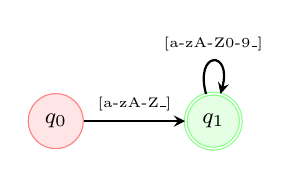
\begin{tikzpicture}[
        state/.style={circle, draw=blue!50, fill=blue!10, minimum size=0.7cm, font=\footnotesize},
        accept/.style={circle, draw=green!50, fill=green!10, minimum size=0.7cm, font=\footnotesize, double},
        start/.style={circle, draw=red!50, fill=red!10, minimum size=0.7cm, font=\footnotesize},
        arrow/.style={->, >=stealth, thick},
        node distance=2cm
    ]
    
    \node[start] (q0) at (0,0) {$q_0$};
    \node[accept] (q1) at (2,0) {$q_1$};
    
    \draw[arrow] (q0) -- node[above, font=\tiny] {[a-zA-Z\_]} (q1);
    \draw[arrow] (q1) to[loop above] node[above, font=\tiny] {[a-zA-Z0-9\_]} (q1);
    
    \end{tikzpicture}%
    }
    \caption{DFA untuk identifier: \texttt{[a-zA-Z\_][a-zA-Z0-9\_]*}}
    \label{fig:identifier-dfa}
\end{figure}

\begin{figure}[H]
    \centering
    \adjustbox{max width=0.5\textwidth,center}{%
    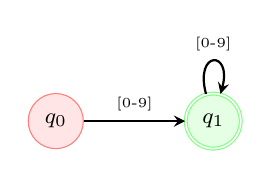
\begin{tikzpicture}[
        state/.style={circle, draw=blue!50, fill=blue!10, minimum size=0.7cm, font=\footnotesize},
        accept/.style={circle, draw=green!50, fill=green!10, minimum size=0.7cm, font=\footnotesize, double},
        start/.style={circle, draw=red!50, fill=red!10, minimum size=0.7cm, font=\footnotesize},
        arrow/.style={->, >=stealth, thick},
        node distance=2cm
    ]
    
    \node[start] (q0) at (0,0) {$q_0$};
    \node[accept] (q1) at (2,0) {$q_1$};
    
    \draw[arrow] (q0) -- node[above, font=\tiny] {[0-9]} (q1);
    \draw[arrow] (q1) to[loop above] node[above, font=\tiny] {[0-9]} (q1);
    
    \end{tikzpicture}%
    }
    \caption{DFA untuk number: \texttt{[0-9]+}}
    \label{fig:number-dfa}
\end{figure}

\begin{lstlisting}[language=C++, caption={Token Recognizer menggunakan DFA}]
enum TokenType {
    IDENTIFIER,
    NUMBER,
    UNKNOWN
};

class TokenRecognizer {
private:
    DFA identifier_dfa;  // DFA untuk [a-zA-Z_][a-zA-Z0-9_]*
    DFA number_dfa;      // DFA untuk [0-9]+
    
public:
    TokenRecognizer() {
        // Konstruksi DFA untuk identifier dan number
        // (dari regex menggunakan Thompson + subset construction)
        buildIdentifierDFA();
        buildNumberDFA();
    }
    
    TokenType recognize(const std::string& lexeme) {
        if (identifier_dfa.simulate(lexeme)) {
            return IDENTIFIER;
        } else if (number_dfa.simulate(lexeme)) {
            return NUMBER;
        } else {
            return UNKNOWN;
        }
    }
    
private:
    void buildIdentifierDFA() {
        // Implementasi konstruksi DFA untuk identifier
        // Regex: [a-zA-Z_][a-zA-Z0-9_]*
    }
    
    void buildNumberDFA() {
        // Implementasi konstruksi DFA untuk number
        // Regex: [0-9]+
    }
};
\end{lstlisting}

Contoh penggunaan:

\begin{lstlisting}[language=C++, caption={Contoh penggunaan TokenRecognizer}]
int main() {
    TokenRecognizer recognizer;
    
    std::vector<std::string> test_inputs = {
        "variable123",  // IDENTIFIER
        "42",           // NUMBER
        "_private",     // IDENTIFIER
        "3.14",         // UNKNOWN (belum support float)
        "123abc"        // UNKNOWN (mixed)
    };
    
    for (const auto& input : test_inputs) {
        TokenType type = recognizer.recognize(input);
        std::cout << input << " -> ";
        switch(type) {
            case IDENTIFIER: std::cout << "IDENTIFIER\n"; break;
            case NUMBER: std::cout << "NUMBER\n"; break;
            case UNKNOWN: std::cout << "UNKNOWN\n"; break;
        }
    }
    
    return 0;
}
\end{lstlisting}

\subsection{Handling Multiple Tokens}

Ketika kita memiliki multiple token types, kita perlu menggabungkan semua pattern menjadi satu DFA. Gambar \ref{fig:multiple-tokens} menunjukkan proses penggabungan NFA untuk multiple token types.

\begin{figure}[H]
    \centering
    \adjustbox{max width=0.85\textwidth,center}{%
    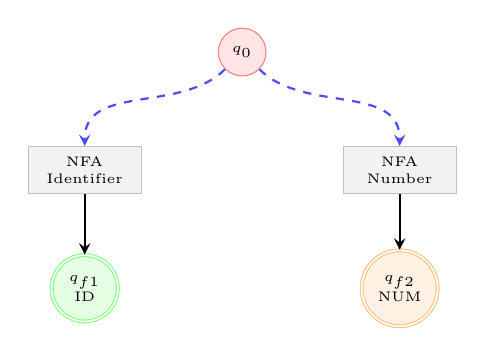
\begin{tikzpicture}[
        state/.style={circle, draw=blue!50, fill=blue!10, minimum size=0.6cm, font=\tiny},
        accept1/.style={circle, draw=green!50, fill=green!10, minimum size=0.6cm, font=\tiny, double, align=center},
        accept2/.style={circle, draw=orange!50, fill=orange!10, minimum size=0.6cm, font=\tiny, double, align=center},
        start/.style={circle, draw=red!50, fill=red!10, minimum size=0.6cm, font=\tiny},
        box/.style={rectangle, draw=gray!50, fill=gray!10, text width=1.2cm, minimum height=0.6cm, font=\tiny, align=center},
        arrow/.style={->, >=stealth, thick},
        eps/.style={->, >=stealth, thick, dashed, blue!70},
        node distance=1.2cm
    ]
    
    \node[start] (q0) at (0,0) {$q_0$};
    \node[box] (nfa1) at (-2,-1.5) {NFA\\Identifier};
    \node[box] (nfa2) at (2,-1.5) {NFA\\Number};
    \node[accept1] (qf1) at (-2,-3) {$q_{f1}$\\ID};
    \node[accept2] (qf2) at (2,-3) {$q_{f2}$\\NUM};
    
    \draw[eps] (q0) to[out=225, in=90] (nfa1);
    \draw[eps] (q0) to[out=315, in=90] (nfa2);
    \draw[arrow] (nfa1) -- (qf1);
    \draw[arrow] (nfa2) -- (qf2);
    
    \end{tikzpicture}%
    }
    \caption{Penggabungan NFA untuk multiple token types dengan labeling accept states}
    \label{fig:multiple-tokens}
\end{figure}

Proses handling multiple tokens:

\begin{enumerate}
    \item Membuat NFA terpisah untuk setiap token type
    \item Menggabungkan semua NFA dengan union, tetapi \textbf{label setiap accept state} dengan token type-nya
    \item Konversi ke DFA (setiap DFA state mungkin mengandung multiple NFA accept states dengan label berbeda)
    \item Saat scanning, jika mencapai accept state dengan multiple labels, gunakan \textbf{priority} atau \textbf{longest match}
\end{enumerate}

Contoh implementasi untuk multiple tokens:

\begin{lstlisting}[language=C++, caption={Handling Multiple Token Types}]
class MultiTokenRecognizer {
private:
    DFA combined_dfa;
    std::map<int, TokenType> state_to_token;
    
public:
    TokenType recognize(const std::string& lexeme) {
        int final_state = combined_dfa.simulate(lexeme);
        if (final_state == -1) return UNKNOWN;
        
        // Jika state memiliki multiple labels, gunakan priority
        if (state_to_token.find(final_state) != state_to_token.end()) {
            return state_to_token[final_state];
        }
        return UNKNOWN;
    }
    
    // Longest match: scan sampai tidak bisa lanjut
    Token scanLongestMatch(std::istream& input) {
        std::string lexeme;
        int last_accept_state = -1;
        int last_accept_pos = -1;
        int current_state = start_state;
        int pos = 0;
        
        char c;
        while (input.get(c)) {
            lexeme += c;
            // Update state dengan input c
            // ...
            
            if (isAcceptState(current_state)) {
                last_accept_state = current_state;
                last_accept_pos = pos;
            }
            pos++;
        }
        
        // Kembalikan ke posisi terakhir yang accept
        input.seekg(last_accept_pos);
        return Token(state_to_token[last_accept_state], 
                     lexeme.substr(0, last_accept_pos + 1));
    }
};
\end{lstlisting}

\section{Optimasi: DFA Minimization}

Setelah subset construction, DFA yang dihasilkan mungkin memiliki states yang redundan. Kita dapat meminimalkan DFA menggunakan algoritma seperti \textbf{Hopcroft's algorithm} atau \textbf{Moore's algorithm}. Gambar \ref{fig:dfa-minimization} menunjukkan contoh DFA sebelum dan sesudah minimisasi.

\begin{figure}[H]
    \centering
    \adjustbox{max width=0.9\textwidth,center}{%
    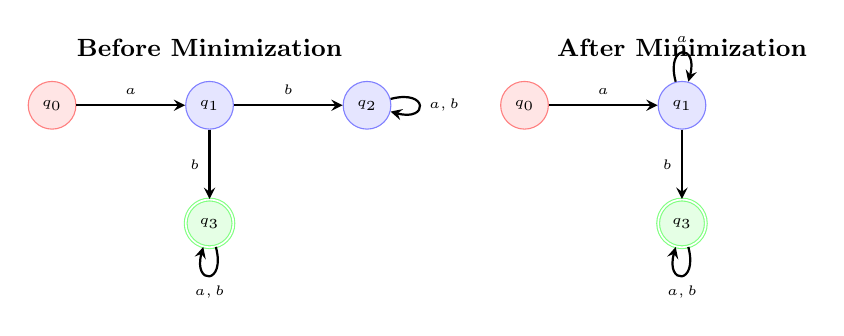
\begin{tikzpicture}[
        state/.style={circle, draw=blue!50, fill=blue!10, minimum size=0.6cm, font=\tiny},
        accept/.style={circle, draw=green!50, fill=green!10, minimum size=0.6cm, font=\tiny, double},
        start/.style={circle, draw=red!50, fill=red!10, minimum size=0.6cm, font=\tiny},
        arrow/.style={->, >=stealth, thick},
        node distance=1.5cm
    ]
    
    % Before minimization
    \node[font=\small, above=0.5cm] at (0,0) {\textbf{Before Minimization}};
    \node[start] (q0a) at (-2,0) {$q_0$};
    \node[state] (q1a) at (0,0) {$q_1$};
    \node[state] (q2a) at (2,0) {$q_2$};
    \node[accept] (q3a) at (0,-1.5) {$q_3$};
    
    \draw[arrow] (q0a) -- node[above, font=\tiny] {$a$} (q1a);
    \draw[arrow] (q1a) -- node[above, font=\tiny] {$b$} (q2a);
    \draw[arrow] (q2a) to[loop right] node[right, font=\tiny] {$a,b$} (q2a);
    \draw[arrow] (q1a) -- node[left, font=\tiny] {$b$} (q3a);
    \draw[arrow] (q3a) to[loop below] node[below, font=\tiny] {$a,b$} (q3a);
    
    % After minimization
    \node[font=\small, above=0.5cm] at (6,0) {\textbf{After Minimization}};
    \node[start] (q0b) at (4,0) {$q_0$};
    \node[state] (q1b) at (6,0) {$q_1$};
    \node[accept] (q3b) at (6,-1.5) {$q_3$};
    
    \draw[arrow] (q0b) -- node[above, font=\tiny] {$a$} (q1b);
    \draw[arrow] (q1b) -- node[left, font=\tiny] {$b$} (q3b);
    \draw[arrow] (q1b) to[loop above] node[above, font=\tiny] {$a$} (q1b);
    \draw[arrow] (q3b) to[loop below] node[below, font=\tiny] {$a,b$} (q3b);
    
    \end{tikzpicture}%
    }
    \caption{Contoh DFA sebelum dan sesudah minimisasi (state $q_2$ dihapus karena equivalent dengan $q_1$)}
    \label{fig:dfa-minimization}
\end{figure}

\subsection{Konsep State Equivalence}

Dua states dalam DFA dikatakan \textbf{equivalent} jika:
\begin{itemize}
    \item Keduanya accept states ATAU keduanya bukan accept states
    \item Untuk setiap input symbol, transisi dari kedua states menuju ke states yang equivalent
\end{itemize}

\subsection{Algoritma Minimization}

Algoritma minimisasi bekerja dengan:
\begin{enumerate}
    \item Partisi states menjadi dua grup: accept states dan non-accept states
    \item Untuk setiap partisi, periksa apakah states dalam partisi tersebut equivalent
    \item Jika tidak equivalent, pisahkan menjadi partisi baru
    \item Ulangi sampai tidak ada partisi yang dapat dipisah lagi
    \item Merge states dalam partisi yang sama
\end{enumerate}

DFA yang sudah diminimalkan memiliki jumlah states minimum yang masih ekuivalen dengan DFA asli.

\section{Contoh Praktis: Implementasi Lengkap}

Sebagai contoh praktis, berikut adalah implementasi lengkap DFA sederhana untuk mengenali identifier dan number:

\begin{lstlisting}[language=C++, caption={Implementasi Lengkap DFA untuk Identifier dan Number}]
#include <iostream>
#include <string>
#include <map>
#include <set>

class SimpleDFA {
private:
    int start_state;
    std::set<int> accept_states;
    std::map<std::pair<int, char>, int> transitions;
    
    bool isLetter(char c) {
        return (c >= 'a' && c <= 'z') || (c >= 'A' && c <= 'Z') || c == '_';
    }
    
    bool isDigit(char c) {
        return c >= '0' && c <= '9';
    }
    
    bool isAlphanumeric(char c) {
        return isLetter(c) || isDigit(c);
    }
    
public:
    SimpleDFA() {
        // DFA untuk identifier: [a-zA-Z_][a-zA-Z0-9_]*
        start_state = 0;
        accept_states.insert(1);
        
        // State 0 -> State 1 dengan letter atau underscore
        for (char c = 'a'; c <= 'z'; c++) {
            transitions[{0, c}] = 1;
            transitions[{1, c}] = 1;  // Loop di state 1
        }
        for (char c = 'A'; c <= 'Z'; c++) {
            transitions[{0, c}] = 1;
            transitions[{1, c}] = 1;
        }
        transitions[{0, '_'}] = 1;
        transitions[{1, '_'}] = 1;
        
        // State 1 -> State 1 dengan digit
        for (char c = '0'; c <= '9'; c++) {
            transitions[{1, c}] = 1;
        }
    }
    
    bool simulate(const std::string& input) {
        int current_state = start_state;
        
        for (char c : input) {
            auto key = std::make_pair(current_state, c);
            if (transitions.find(key) == transitions.end()) {
                return false;
            }
            current_state = transitions[key];
        }
        
        return accept_states.find(current_state) != accept_states.end();
    }
};

int main() {
    SimpleDFA dfa;
    
    std::vector<std::string> test_cases = {
        "variable",
        "var123",
        "_private",
        "123var",      // Invalid (dimulai dengan digit)
        "var_name",
        "VarName123"
    };
    
    std::cout << "Testing DFA untuk Identifier:\n";
    std::cout << "==============================\n";
    for (const auto& test : test_cases) {
        bool result = dfa.simulate(test);
        std::cout << "\"" << test << "\" -> " 
                  << (result ? "ACCEPT" : "REJECT") << "\n";
    }
    
    return 0;
}
\end{lstlisting}

Output program di atas:

\begin{verbatim}
Testing DFA untuk Identifier:
==============================
"variable" -> ACCEPT
"var123" -> ACCEPT
"_private" -> ACCEPT
"123var" -> REJECT
"var_name" -> ACCEPT
"VarName123" -> ACCEPT
\end{verbatim}

\section{Kesimpulan}

Dalam bab ini, kita telah mempelajari:

\begin{enumerate}
    \item Regular expression adalah notasi formal untuk mendeskripsikan pola token
    \item Finite automata (NFA dan DFA) adalah model matematika untuk mengenali regular language
    \item Algoritma Thompson mengkonversi regular expression menjadi $\epsilon$-NFA
    \item Subset construction mengkonversi NFA menjadi DFA yang ekuivalen
    \item DFA lebih efisien untuk simulasi dan digunakan dalam lexical analysis
    \item Implementasi praktis memerlukan struktur data yang tepat dan algoritma yang efisien
\end{enumerate}

Pemahaman tentang regular expression dan finite automata ini menjadi dasar penting untuk implementasi lexical analyzer yang akan dipelajari dalam bab-bab selanjutnya.

\section{Latihan}

\begin{enumerate}
    \item Buatlah regular expression untuk:
    \begin{itemize}
        \item Email address sederhana (format: \texttt{user@domain.com})
        \item Phone number (format: \texttt{+62-812-3456-7890})
        \item C-style comment (\texttt{/* ... */})
    \end{itemize}
    
    \item Konstruksi NFA untuk regular expression berikut menggunakan algoritma Thompson:
    \begin{itemize}
        \item \texttt{a*b+}
        \item \texttt{(a|b)*ab}
        \item \texttt{[0-9]+(\textbackslash.[0-9]+)?}
    \end{itemize}
    
    \item Konversi NFA dari soal nomor 2 menjadi DFA menggunakan subset construction. Gambarkan state diagram untuk DFA yang dihasilkan.
    
    \item Implementasikan kelas \texttt{NFA} dan \texttt{DFA} dalam C++ dengan fungsi:
    \begin{itemize}
        \item Konstruksi NFA dari regular expression (sederhana)
        \item Konversi NFA ke DFA
        \item Simulasi DFA untuk string input
    \end{itemize}
    
    \item Buat program recognizer yang dapat mengenali token-token berikut:
    \begin{itemize}
        \item Identifier: \texttt{[a-zA-Z\_][a-zA-Z0-9\_]*}
        \item Integer: \texttt{[0-9]+}
        \item Float: \texttt{[0-9]+\textbackslash.[0-9]+}
        \item Operator: \texttt{+|-|*|/|=|==|!=}
    \end{itemize}
    
    \item Jelaskan mengapa DFA lebih efisien untuk simulasi dibanding NFA. Berikan contoh kompleksitas waktu untuk keduanya.
    
    \item Implementasikan algoritma minimisasi DFA (dapat menggunakan versi sederhana). Uji dengan DFA yang dihasilkan dari soal nomor 3.
\end{enumerate}

\section{Referensi dan Bahan Bacaan Lanjutan}

Untuk memperdalam pemahaman tentang regular expression dan finite automata, mahasiswa disarankan membaca:

\begin{itemize}
    \item \textbf{Dragon Book}: Aho, Lam, Sethi, \& Ullman (2006). \textit{Compilers: Principles, Techniques, and Tools} \cite{aho2006compilers} - Bab 3: Lexical Analysis
    
    \item \textbf{Engineering a Compiler}: Cooper \& Torczon (2011) \cite{cooper2011engineering} - Bab 2: Scanners
    
    \item \textbf{Aoyama Gakuin University}: Lecture notes tentang lexical analysis dan finite automata \cite{aoyama2024lexical}
    
    \item \textbf{OpenGenus}: Tutorial tentang membangun lexer \cite{opengenus2024lexer}
    
    \item \textbf{GeeksforGeeks}: Artikel tentang regular expression to NFA dan NFA to DFA conversion
\end{itemize}
